\documentclass[twoside]{article}

% We add packages, macros here:
%!TEX root =  lec-template.tex
\usepackage{lmodern}
\usepackage[english]{babel}
\usepackage{latexsym}
\usepackage{amsmath}
\usepackage{mathrsfs}
\usepackage{amssymb}
\usepackage{mathtools}
\usepackage[inline,shortlabels]{enumitem} % we prefer enumitem because of its margin adjustment caps
\usepackage{bm}
\usepackage{datetime}
\usepackage[table,xcdraw]{xcolor}
\usepackage{accents}
\usepackage{tikz}
\usepackage{listings}
\usepackage{mdframed}
\usepackage{pgfplots}
\usepackage{pgfplotstable}
\usepackage[boxed]{algorithm}
\usepackage{algpseudocode}
\usepackage{dsfont}
\usepackage{color}
\usepackage{colortbl}
\usepackage{pifont}
\usepackage[bf,font=small,singlelinecheck=off]{caption}
\usepackage{microtype} % improved spacing between words for easier reading
\usepackage{float}
\usepackage{xfrac} % sfrac
\usepackage{xspace}

\linespread{1.1}


\usepackage[textsize=tiny]{todonotes}
\makeatletter
\renewcommand{\todo}[2][]{\@todo[#1]{#2}}
\makeatother

\setlength{\marginparwidth}{10ex}
\newcommand{\todoc}[2][]{\todo[size=\scriptsize,color=blue!20!white,#1]{Csaba: #2}}
\newcommand{\todoj}[2][]{\todo[size=\scriptsize,color=red!20!white,#1]{Jincheng: #2}}

\usepackage{hyperref}
\hypersetup{
    unicode=false,          % non-Latin characters in Acrobat�s bookmarks
    pdftoolbar=true,        % show Acrobat�s toolbar?
    pdfmenubar=true,        % show Acrobat�s menu?
    pdffitwindow=false,     % window fit to page when opened
    pdfstartview={FitH},    % fits the width of the page to the window
    pdftitle={},    % title
    pdfauthor={},     % author
    pdfsubject={Theory, Machine Learning, Lectures},   % subject of the document
    pdfcreator={},   % creator of the document
    pdfproducer={}, % producer of the document
    pdfkeywords={theory} {machine learning} {lecture notes} {CMPUT 654} {Fall 2023}, % list of keywords
    pdfnewwindow=true,      % links in new window
    colorlinks=true,       % false: boxed links; true: colored links
    linkcolor=blue,          % color of internal links (change box color with linkbordercolor)
    citecolor=blue,        % color of links to bibliography
    filecolor=magenta,      % color of file links
    urlcolor=cyan           % color of external links
}
\usepackage{amsthm}
\usepackage{times}
\usepackage{natbib}
\usepackage{nicefrac}
\usepackage{wrapfig}
\usepackage[capitalize]{cleveref}
\usepackage[nottoc,numbib]{tocbibind}

%\usepackage[bmargin=0.75in]{geometry}
\usepackage[margin=1.1in]{geometry}
\usepackage[normalem]{ulem}


%%%%%%%%%%%%%%%%%%%%%%%%%%%%%%%%
% HYPHENATION
%%%%%%%%%%%%%%%%%%%%%%%%%%%%%%%%

\pretolerance=5000
\tolerance=9000
\emergencystretch=0pt
\righthyphenmin=4
\lefthyphenmin=4


\bibliographystyle{plainnat}

\newcommand{\E}{\mathbb{E}}
\newcommand{\EE}[1]{\E[#1]}
\newcommand{\PP}{\mathbb{P}}
\newcommand{\Prob}[1]{\mathbb{P}(#1)}
\newcommand{\one}[1]{\mathbb{I}\{#1\}}
\newcommand{\Supp}{\operatorname{supp}}
\newcommand{\ip}[1]{\langle #1 \rangle}
\newcommand{\bip}[1]{\left\langle #1 \right\rangle}
\newcommand{\norm}[1]{\|#1\|}
\newcommand{\R}{\mathbb{R}}
\newcommand{\N}{\mathbb{N}}
\newcommand{\cA}{\mathcal{A}}
\newcommand{\cB}{\mathcal{B}}
\newcommand{\cC}{\mathcal{C}}
\newcommand{\cD}{\mathcal{D}}
\newcommand{\cE}{\mathcal{E}}
\newcommand{\cF}{\mathcal{F}}
\newcommand{\cG}{\mathcal{G}}
\newcommand{\cH}{\mathcal{H}}
\newcommand{\cK}{\mathcal{K}}
\newcommand{\cL}{\mathcal{L}}
\newcommand{\cN}{\mathcal{N}}
\newcommand{\cP}{\mathcal{P}}
\newcommand{\cQ}{\mathcal{Q}}
\newcommand{\cR}{\mathcal{R}}
\newcommand{\cS}{\mathcal{S}}
\newcommand{\sA}{\mathscr A}

\newcommand{\cM}{\mathcal{M}}
\newcommand{\cX}{\mathcal{X}}
\newcommand{\cY}{\mathcal{Y}}
\newcommand{\NN}{\mathbb{N}}
\newcommand{\RR}{\mathbb{R}}
\newcommand{\VV}[1]{\mathbb{V}[#1]}

\newcommand{\epsapp}{\epsilon}
\newcommand{\epssub}{\delta}

\DeclareMathOperator{\Range}{range}
\newcommand{\rows}{\operatorname{rows}}

\renewcommand{\epsilon}{\varepsilon}
\newcommand{\ceil}[1]{\left\lceil {#1} \right\rceil}
\newcommand{\floor}[1]{\left\lfloor {#1} \right\rfloor}
\newcommand{\ones}{\mathbf{1}}
\newcommand{\zeros}{\mathbf{0}}
\DeclareMathOperator*{\argmin}{arg\ min}
\DeclareMathOperator*{\argmax}{arg\ max}


\def\rvzero{{\mathbf{0}}}
\def\rvone{{\mathbf{1}}}

\def\identiymatrix{\mathbf{Id}}

\newcommand{\softmax}{\mathrm{softmax}}
\newcommand{\KL}{D_{\mathrm{KL}}}

% Graph
\def\gA{{\mathcal{A}}}
\def\gB{{\mathcal{B}}}
\def\gC{{\mathcal{C}}}
\def\gD{{\mathcal{D}}}
\def\gE{{\mathcal{E}}}
\def\gF{{\mathcal{F}}}
\def\gG{{\mathcal{G}}}
\def\gH{{\mathcal{H}}}
\def\gI{{\mathcal{I}}}
\def\gJ{{\mathcal{J}}}
\def\gK{{\mathcal{K}}}
\def\gL{{\mathcal{L}}}
\def\gM{{\mathcal{M}}}
\def\gN{{\mathcal{N}}}
\def\gO{{\mathcal{O}}}
\def\gP{{\mathcal{P}}}
\def\gQ{{\mathcal{Q}}}
\def\gR{{\mathcal{R}}}
\def\gS{{\mathcal{S}}}
\def\gT{{\mathcal{T}}}
\def\gU{{\mathcal{U}}}
\def\gV{{\mathcal{V}}}
\def\gW{{\mathcal{W}}}
\def\gX{{\mathcal{X}}}
\def\gY{{\mathcal{Y}}}
\def\gZ{{\mathcal{Z}}}

% Sets
\def\sA{{\mathbb{A}}}
\def\sB{{\mathbb{B}}}
\def\sC{{\mathbb{C}}}
\def\sD{{\mathbb{D}}}
% Don't use a set called E, because this would be the same as our symbol
% for expectation.
\def\sE{{\mathbb{E}}}
\def\sF{{\mathbb{F}}}
\def\sG{{\mathbb{G}}}
\def\sH{{\mathbb{H}}}
\def\sI{{\mathbb{I}}}
\def\sJ{{\mathbb{J}}}
\def\sK{{\mathbb{K}}}
\def\sL{{\mathbb{L}}}
\def\sM{{\mathbb{M}}}
\def\sN{{\mathbb{N}}}
\def\sO{{\mathbb{O}}}
\def\sP{{\mathbb{P}}}
\def\sQ{{\mathbb{Q}}}
\def\sR{{\mathbb{R}}}
\def\sS{{\mathbb{S}}}
\def\sT{{\mathbb{T}}}
\def\sU{{\mathbb{U}}}
\def\sV{{\mathbb{V}}}
\def\sW{{\mathbb{W}}}
\def\sX{{\mathbb{X}}}
\def\sY{{\mathbb{Y}}}
\def\sZ{{\mathbb{Z}}}

\newcommand{\dimE}{\mathrm{dim}_{\mathcal{E}}}
\DeclareMathOperator{\diam}{diam}


%%
%% ADD PACKAGES here:
%%
%
%\usepackage{amsmath,amsfonts,graphicx}
%
%
% The following commands set up the lecnum (lecture number)
% counter and make various numbering schemes work relative
% to the lecture number.
%

\newcounter{lecnum}
\renewcommand{\thepage}{\thelecnum-\arabic{page}}
\renewcommand{\thesection}{\thelecnum.\arabic{section}}
\renewcommand{\theequation}{\thelecnum.\arabic{equation}}
\renewcommand{\thefigure}{\thelecnum.\arabic{figure}}
\renewcommand{\thetable}{\thelecnum.\arabic{table}}


%
% The following macro is used to generate the header.
%
\newcommand{\lecture}[4]{
   \pagestyle{myheadings}
   \thispagestyle{plain}
   \newpage
   \setcounter{lecnum}{#1}
   \setcounter{page}{1}
   \noindent
   \begin{center}
   \framebox{
      \vbox{\vspace{2mm}
    \hbox to 6.28in { {\bf CMPUT 654 Fa 23: Theoretical Foundations of Machine Learning \hfill Fall 2023} }
       \vspace{4mm}
       \hbox to 6.28in { {\Large \hfill Lecture #1: #2  \hfill} }
       \vspace{2mm}
       \hbox to 6.28in { {\it Lecturer: #3 \hfill Scribes: #4} }
      \vspace{2mm}}
   }
   \end{center}
   \markboth{Lecture #1: #2}{Lecture #1: #2}

   \noindent {\bf Note}: {\it 
   \LaTeX\  template courtesy of UC Berkeley EECS dept. (\href{https://inst.eecs.berkeley.edu/~cs294-8/sp03/Materials/}{link} to directory)
   }

   \noindent {\bf Disclaimer}: {\it These notes have \underline{\textbf{not}} been subjected to the
   usual scrutiny reserved for formal publications. They may be
   distributed outside this class only with the permission of the
   Instructor.} \vspace*{4mm}
}
%
% Convention for citations is authors' initials followed by the year.
% For example, to cite a paper by Leighton and Maggs you would type
% \cite{LM89}, and to cite a paper by Strassen you would type \cite{S69}.
%%%%%%%%% (To avoid bibliography problems, for now we redefine the \cite command.)
%%%%%%%%% Also commands that create a suitable format for the reference list.
%%%%%%%%\renewcommand{\cite}[1]{[#1]}
%%%%%%%%\def\beginrefs{\begin{list}%
%%%%%%%%        {[\arabic{equation}]}{\usecounter{equation}
%%%%%%%%         \setlength{\leftmargin}{2.0truecm}\setlength{\labelsep}{0.4truecm}%
%%%%%%%%         \setlength{\labelwidth}{1.6truecm}}}
%%%%%%%%\def\endrefs{\end{list}}
%%%%%%%%\def\bibentry#1{\item[\hbox{[#1]}]}

%Use this command for a figure; it puts a figure in wherever you want it.
%usage: \fig{NUMBER}{SPACE-IN-INCHES}{CAPTION}
\newcommand{\fig}[3]{
			\vspace{#2}
			\begin{center}
			Figure \thelecnum.#1:~#3
			\end{center}
	}
% Use these for theorems, lemmas, proofs, etc.

%!TEX root =  lec-template.tex
%%%%%%%%%%%%%%%%%%%%%%%%%%%%%%%%
% THEOREMS
%%%%%%%%%%%%%%%%%%%%%%%%%%%%%%%%
\theoremstyle{plain}
\newtheorem{theorem}{Theorem}[lecnum]
\newtheorem{claim}[theorem]{Claim}
\newtheorem{proposition}[theorem]{Proposition}
\newtheorem{lemma}[theorem]{Lemma}
\newtheorem{corollary}[theorem]{Corollary}
\newtheorem{example}[theorem]{Example}
\theoremstyle{definition}
\newtheorem{definition}[theorem]{Definition}
\newtheorem{assumption}[theorem]{Assumption}
\newtheorem{remark}[theorem]{Remark}
\newtheorem{exercise}[theorem]{Exercise}
\theoremstyle{remark}


%\newtheorem{theorem}{Theorem}[lecnum]
%\newtheorem{lemma}[theorem]{Lemma}
%\newtheorem{proposition}[theorem]{Proposition}
%\newtheorem{claim}[theorem]{Claim}
%\newtheorem{corollary}[theorem]{Corollary}
%\newtheorem{definition}[theorem]{Definition}
%\newenvironment{proof}{{\bf Proof:}}{\hfill\rule{2mm}{2mm}}

% **** IF YOU WANT TO DEFINE ADDITIONAL MACROS FOR YOURSELF, PUT THEM HERE:

\newcommand{\set}[1]{\left\{#1\right\}}
\newcommand{\I}{\mathbb{I}}
\newcommand{\cW}{\mathcal{W}}

\begin{document}
%FILL IN THE RIGHT INFO.
% \lecture{**LECTURE-NUMBER**}{**DATE**}{**LECTURER**}{**SCRIBE**}
\lecture{20}{Kernel Methods (November 21)}{Csaba Szepesv\'ari}{Kushagra Chandak}
%\footnotetext{These notes are partially based on those of Nigel Mansell.}

\newcommand{\Rad}{\mathrm{Rad}}

% **** YOUR NOTES GO HERE:

% Some general latex examples and examples making use of the
% macros follow.  
%**** IN GENERAL, BE BRIEF. LONG SCRIBE NOTES, NO MATTER HOW WELL WRITTEN,
%**** ARE NEVER READ BY ANYBODY.

\paragraph{Motivation.}
Suppose we have a feature map 
\[
\psi: \cX \to \R^d
\]
which is used to make predictions 
\[
f_w(x) = \ip{w, \psi(x)}\,,
\]
where $w \in \R^d$. Note that if $d$ is huge then computing the prediction $f_w(x)$ is expensive (linear in $d$). Can we do this efficiently? Ambitiously, can we replace $\R^d$ with some \emph{Hilbert space} $\cW$? Recall that a Hilbert space is a complete inner product space. The endowed inner product is a bilinear function $\ip{\cdot, \cdot}: \cW^2 \to \R$ satisfying the following properties for any $u, v, u_1, u_2 \in \cW$.
\begin{enumerate}
    \item (Symmetric) $\ip{u, v} = \ip{v, u}$.
    \item (Linear in both arguments) $\ip{u_1 + u_2, v} = \ip{u_1, v} + \ip{u_2, v}$ and $\ip{\lambda u, v} = \lambda \ip{u, v}$.
    \item (Positive) $\ip{u, u} = 0$ iff $u = 0$
\end{enumerate}
Note that the inner product induces the norm $\norm{u}^2 = \ip{u, u}$. Some examples of Hilbert spaces:
\begin{enumerate}
    \item $\cW = \R^d$ with the inner product of the form $\ip{u, v} = u^\top Q v$ where $Q$ is PSD ($Q \succeq 0$).
    \item $\cW = \ell_2(\R^\NN)$, where $\ell_2(\R^\NN) \subset \R^N$ such that $\norm{u}^2 = \sum_{i=1}^\infty u_i^2 < \infty$ for all $u \in \cW$, with the inner product $\sum_{i=1}^\infty u_i  v_i$. 
\end{enumerate}
With a Hilbert space structure, we can do computations like calculating ERM efficiently. We have input space $\cX$ and output space $\cY$. The prediction we want to compute efficiently is $f_w(x) = \ip{w, \psi(x)}$. We also have a loss function $\ell : \R \times \cY \to \R$. For data $(x_1, y_1), \dots, (x_n, y_n) \in \cX \times \cY$, the regularized loss is defined as
\begin{align*}\label{eq:loss-w}
       Q(w) = \frac1n \sum_{i=1}^n \ell(f_w(x_i), y_i) + \frac\lambda2 \norm{w}^2 \,.
\end{align*}
 
We introduce another map, the \emph{kernel}, $k:\cX^2 \to \R$, using which we can write the ERM solution.
\[
    k(u,v) = \ip{\psi(u), \psi(v)}\,.
\]
Now imagining that the Hilbert space $\cW$ is $\R^d$, we can find the ERM solution:
\[
    0 = Q'(w) = \frac1n \sum_{i=1}^n \frac{\partial }{\partial p} \ell(f_w(x_i), y_i) \psi(x_i) + \lambda w \,,
\]
or
\begin{align*}
    w  =  - \frac{1}{\lambda n} \sum_{i=1}^n \frac{\partial }{\partial p} \ell(f_w(x_i), y_i) \psi(x_i) = \sum_{i=1}^n \alpha_i \psi(x_i) \,.
\end{align*}
Therefore $f_w$ can be computed as
\begin{align*}
    f_w(x) = \ip{w, \psi(x)} = \sum_{i=1}^n \alpha_i k(x_i, x) = \tilde f_\alpha(x), \quad \alpha \in \R^n\,.
\end{align*}
Note that the penalty term $\norm{w}^2$ can be written as
\[
    \norm{w}^2 = \sum_{i, j=1}^n \alpha_i \alpha_j k(x_i, x_j) = \alpha^\top K \alpha\,,
\]
where $K$ is an $n \times n$ matrix composed from the kernel: $K = (k(x_i, x_j)_{i,j=1}^n$.

We can also optimize the loss in the $\alpha$ ($\R^n$) space:
\begin{align*}\label{eq:loss-alpha}
    \tilde Q(\alpha) = \frac1n \sum_{i=1}^n \ell(\tilde f_\alpha(x_i), y_i) + \frac\lambda2 \alpha^\top K \alpha
\end{align*}

We can go between the $\alpha$ space ($\R^n$) and the $\cW$ space. Going from $\R^n$ to $\cW$ is simpler, and can be done using the map $\phi: \R^n \to \cW$ defined as $\alpha \mapsto \sum_{i=1}^n \alpha_i \psi(x_i)$. 


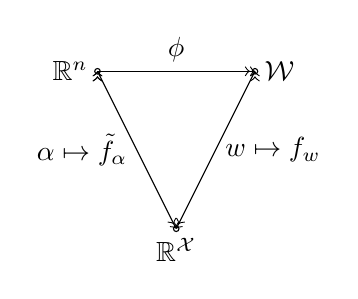
\begin{tikzpicture}
\draw[] (0,0) circle (1pt) node[anchor=east]{$\R^n$};
\draw[] (2,0) circle (1pt) node[anchor=west]{$\cW$};
\draw[] (1,-2) circle (1pt) node[anchor=north]{$\R^\cX$};

\draw[->>] (0,0) edge node[above] {$\phi$} (2,0);
\draw[->>] (2,0) edge node[right] {$w \mapsto f_w$} (1,-2);
\draw[->>] (0,0) edge node[left] {$\alpha \mapsto \tilde f_\alpha$} (1,-2);
\end{tikzpicture}

We know that $\phi(\R^n) \subset \cW$. So if we can show that $\argmin_{w \in \cW} Q(w) \subset \phi(\R^n)$ then minimizing $Q(w)$ would be same as minimizing $\tilde Q(\alpha)$. 


Switching to the ``$\alpha$'' representation is called the \emph{kernel trick}. 


\begin{definition}[Positive definite kernel\footnote{Technically, positive semi-definite}]
    Let $k: \cX^2 \to \R$ be symmetric. $k$ is positive definite if for all $n \in \NN$, $x_{1:n} \in \cX^n$ and $\alpha \in \R^n$, $\sum_{i=1}^n \sum_{j=1}^n \alpha_i \alpha_j k(x_i, x_j) \ge 0$.
\end{definition}

Let $k$ be a symmetric positive definite kernel. Let $\cH_0 \subseteq \R^\cX$ be defined by
\[
    \cH_0 = \set{x \mapsto \sum_{i=1}^n \alpha_i k(x, x_i) : n \in \NN, \alpha \in \R^n}\,.
\]
Suppose we define a function on $\cH_0$ (which we will claim to be an inner product)
\[
\ip{\sum_{i=1}^n \alpha_i k(x_i, \cdot), \sum_{j=1}^n \beta_j k(x_j, \cdot)} = \sum_{i=1}^n \sum_{j=1}^n \alpha_i \beta_j k(x_i, x_j) \,.
\]

\begin{claim}
    $\cH_0$ is a pre-Hilbert space (no completeness).
\end{claim}

\begin{theorem}
    For every symmetric positive definite $k$,  $\exists ! (\cH, \ip{\cdot, \cdot} \subseteq \R^\cX$ Hilbert space such that $\cH_0 \subseteq \cH$ is dense. For any function $\sum \alpha_i k(x_i, \cdot), \beta_j k(x_j, \cdot) \in \cH_0$, $\ip{\alpha_i k(x_i, \cdot), \beta_j k(x_j, \cdot)} = \sum_{i,j} \alpha_i \beta_j k(x_i, x_j)$.
\end{theorem}
The space $\cH$ is called a \emph{reproducing kernel Hilbert space} (RKHS). A RKHS has the \emph{reproducing kernel} property which follows from the construction:
\[
    f(x) = \ip{f, k(x,\cdot)} \,.
\]
 
\end{document}
